\documentclass[11pt,a4paper,oneside]{report}

% Lingua e codifica
\usepackage[italian]{babel}
\usepackage[utf8]{inputenc}
\usepackage[T1]{fontenc}

% Pacchetti aggiuntivi necessari
\usepackage{float}
\usepackage{booktabs}
\usepackage{amsmath}
\usepackage{graphicx}
\usepackage{caption}
\usepackage{subcaption}

% Impaginazione compatta
\usepackage[a4paper,top=1.6cm,bottom=1.8cm,left=1.6cm,right=1.6cm]{geometry}
\usepackage{setspace}
\setstretch{1.0}
\setlength{\parskip}{4pt}
\setlength{\parindent}{0pt}

\begin{document}

% =========================
% PRIMA PAGINA COMPATTA
% =========================
\begin{titlepage}
    \centering
    {\large Università degli Studi di Brescia\par}
    {\normalsize Laboratorio di Automatica -- A.A. 2025/2026\par}
    \vspace{1.2cm}

    {\LARGE \textbf{Relazione Tecnica}\par}
    \vspace{0.2cm}
    {\Large Assignment 1 -- Gantry Crane con SEA\par}
    \vspace{1cm}

    {\normalsize \textbf{Gruppo:} 30\par}
    {\normalsize \textbf{Componente:} Alessandro Vigorelli\par}

    \vspace{1.2cm}
    {\normalsize \textbf{Introduzione}\par}
Questo documento riassume il lavoro svolto per la prima parte dell'elaborato richiesto nel corso di Laboratorio di Automatica,
dedicato al controllo di un sistema gantry con attuatori elastici in serie (SEA) in ambiente di simulazione. 
L'obiettivo generale è ottenere un controllo stabile e robusto, che riesca a seguire la traiettoria attraverso degli ostacoli posti nel minor tempo 
possibile senza collisioni.

\textbf{Obiettivi principali:}
\begin{itemize}
    \item identificare i modelli dinamici dei tre giunti mediante test con segnale chirp;
    \item validare i modelli ottenuti confrontando la risposta identificata con i dati simulati;
    \item progettare e tarare il controllo in cascata, composto da anello interno di velocità
    e anello esterno di posizione;
    \item introdurre filtri low-pass e notch per attenuare rumore e risonanze elastiche;
    \item integrare la compensazione feedforward tramite parametri dinamici identificati;
    \item aumentare progressivamente velocità e accelerazione mantenendo stabilità,
    accuratezza e robustezza;
    \item valutare quantitativamente le prestazioni tramite errori di inseguimento,
    tempo ciclo e sollecitazioni massime.
\end{itemize}

Il problema tecnico centrale consiste nel bilanciare aggressività del controllo e precisione: aumentando velocità, accelerazione
 si riduce il tempo ciclo, ma cresce il rischio di oscillazioni, 
sensibilità al rumore e perdita di accuratezza locale lungo il percorso tra degli ostacoli. 
Nelle sezioni successive verranno presentati metodo, risultati sperimentali in simulazione 
e criteri di scelta della configurazione finale.
\end{titlepage}

\section{Identificazione e validazione dei modelli}
\label{sec:ident_valid}

L'identificazione dei modelli dei tre giunti è stata svolta mediante prove in frequenza con 
segnale chirp, utilizzando come ingresso l'ampiezza del segnale e come uscita la velocità del giunto.  
Per ogni prova sono stati variati i parametri principali del test 
(banda del chirp, durata, ampiezza e pesatura in frequenza), con successiva validazione dei modelli ottenuti.

La validazione è stata condotta confrontando la risposta in frequenza del modello 
identificato con la funzione di Risposta in Frequenza sperimentale ottenuta da prove indipendenti, analizzando la
coerenza di modulo e fase,la capacità di riprodurre correttamente anti-risonanze e 
risonanze e la robustezza del modello rispetto a differenti condizioni di prova.

\subsection*{Tabella riepilogo prove di identificazione}
\begin{table}[H]
    \centering
    \footnotesize
    \caption{Riepilogo test di identificazione e parametri di stima.}
    \label{tab:ident_tests}
    \makebox[\linewidth][c]{
    \begin{tabular}{lccccccccc}
    \toprule
    \textbf{Test} & \textbf{Giunto} & \textbf{Ampiezza} & \textbf{$f_0$ [Hz]} & \textbf{$f_1$ [Hz]} & \textbf{Tempo [s]} & \textbf{Pesi usati} & \textbf{$\omega_{ar}$ [rad/s]} & \textbf{$\omega_r$ [rad/s]} & \textbf{model\_ord} \\
    \midrule
    T01 & J1 & 40 & 0.1 & 500 & 60  & [20, 2700] & 300 & 650 & 3\\
    T02 & J2 & 40 & 0.1 & 500 & 60  & [20, 2700] & 350 & 800 & 3\\
    T03 & J3 & 40 & 0.1 & 500 & 60  & [20, 2700] & 550 & 750 & 3\\
    T04 & J3 & 15 & 0.1 & 300 & 120 & [20, 1500] & 550 & 750 & 4\\
    \bottomrule
    \end{tabular}
    }
\end{table}

\vspace{-0.4cm}
\begin{figure}[H]
    \makebox[\linewidth][c]{
        \begin{subfigure}[b]{0.56\textwidth}
            \centering
            \scalebox{1}[1.1]{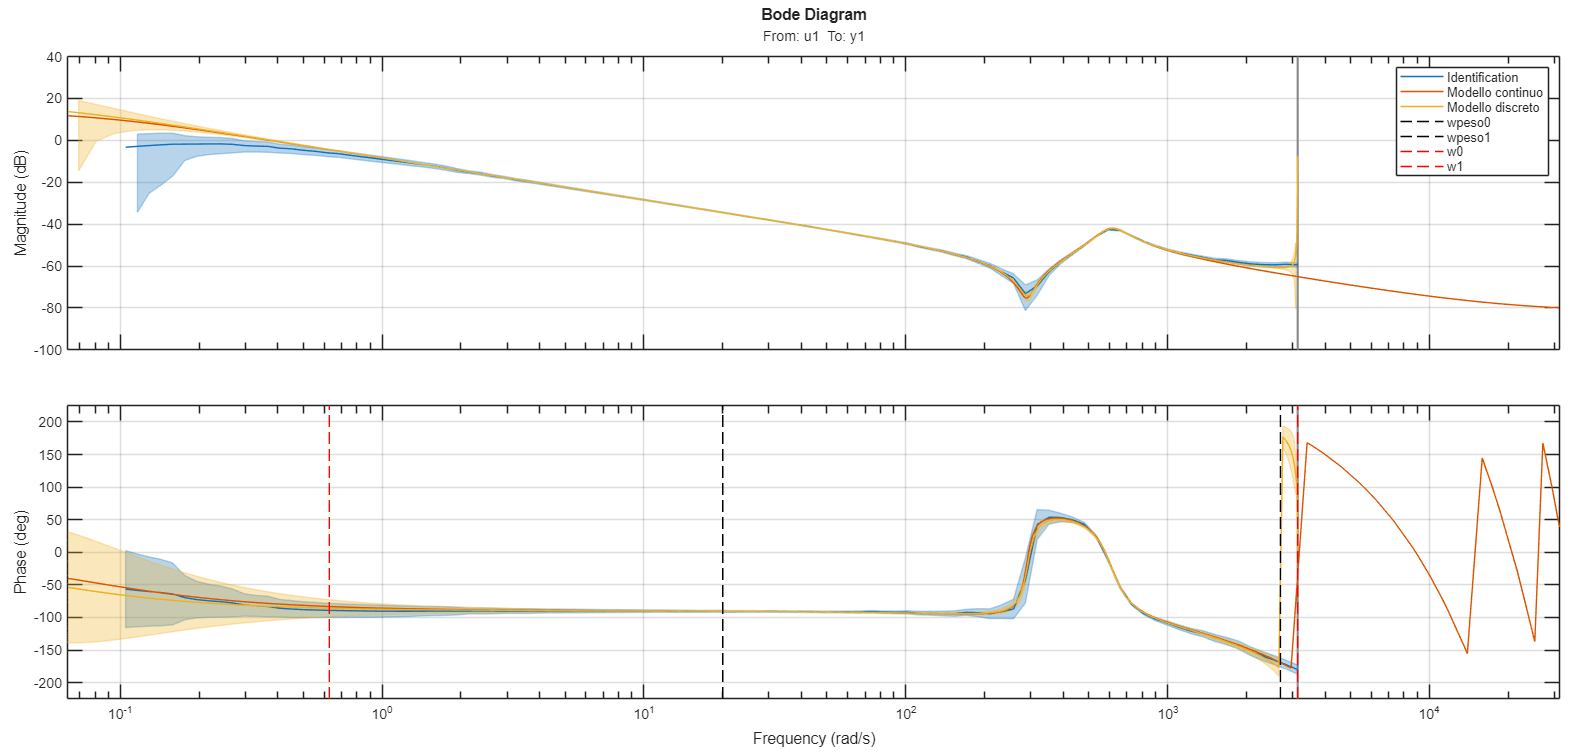
\includegraphics[width=\textwidth]{IMG/ident_valid/J1_IDENTIF.png}}
            \caption{Giunto J1 (T01)}
            \label{fig:j1_ident}
        \end{subfigure}
        \hspace{0.02\textwidth}
        \begin{subfigure}[b]{0.56\textwidth}
            \centering
            \scalebox{1}[1.1]{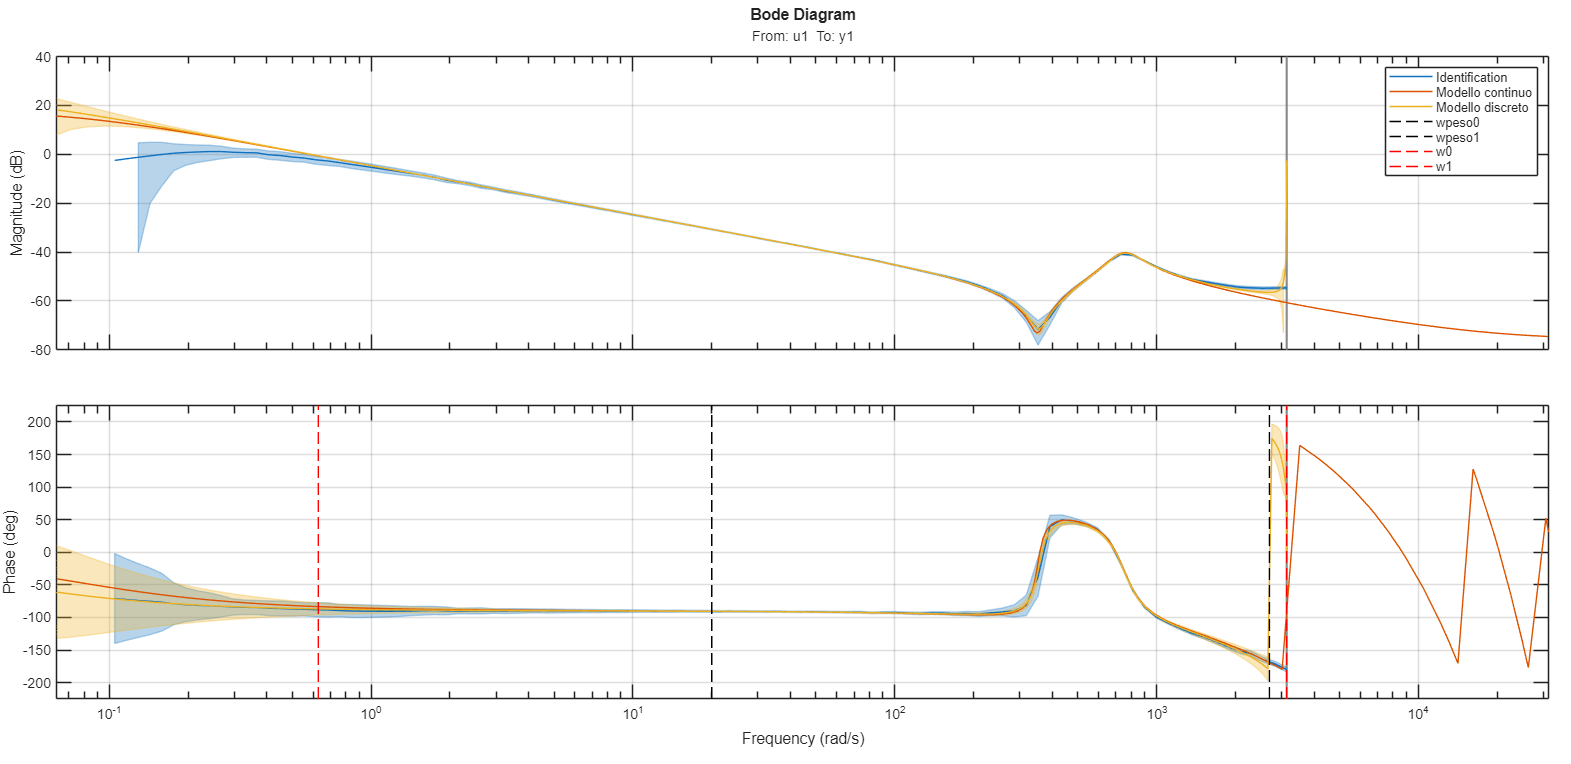
\includegraphics[width=\textwidth]{IMG/ident_valid/J2_IDENTIF.png}}
            \caption{Giunto J2 (T02)}
            \label{fig:j2_ident}
        \end{subfigure}
    }
    
    \vspace{-0.1cm}
    
    \makebox[\linewidth][c]{
        \begin{subfigure}[b]{0.56\textwidth}
            \centering
            \scalebox{1}[1.1]{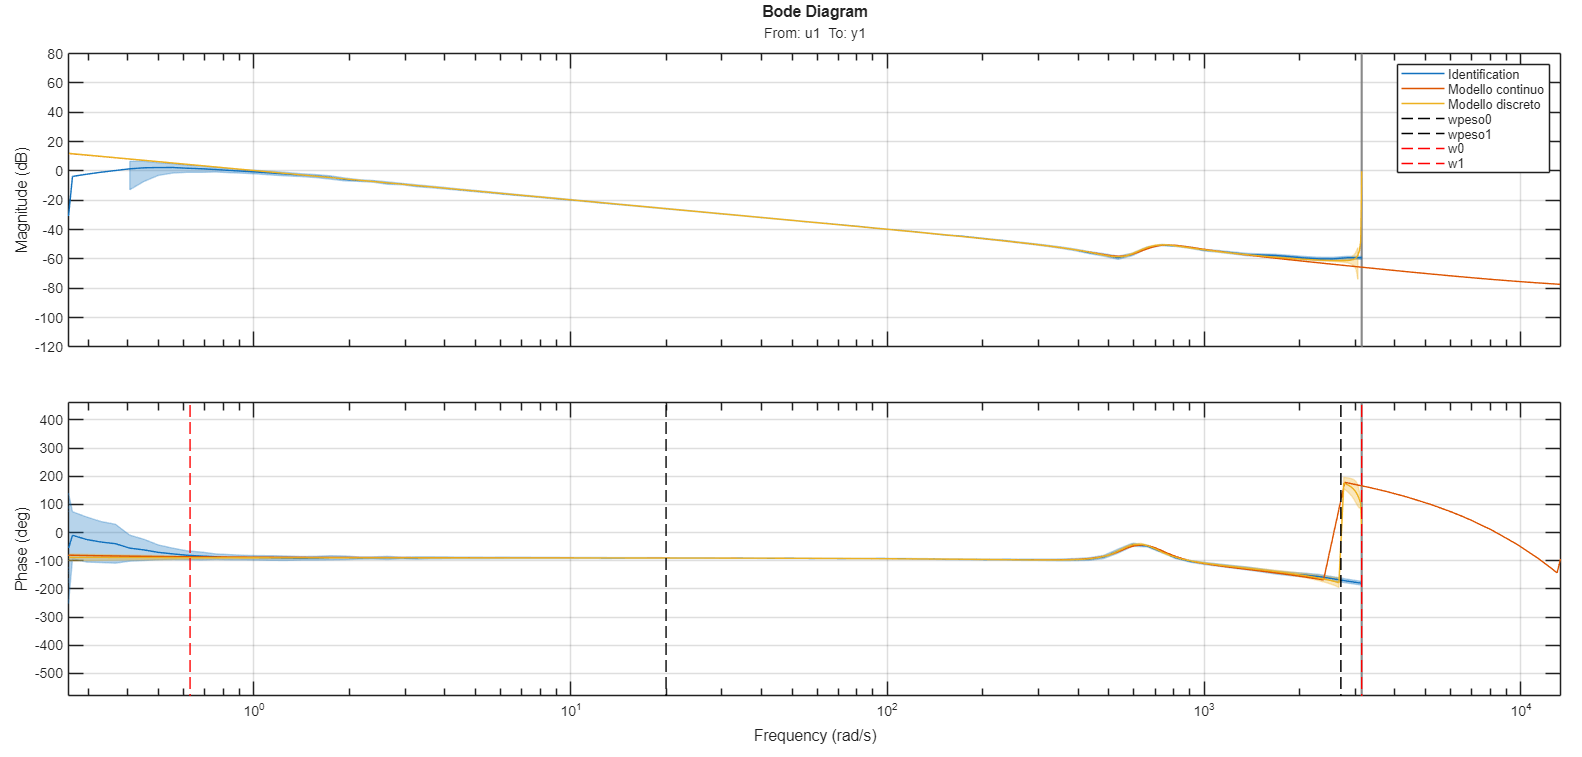
\includegraphics[width=\textwidth]{IMG/ident_valid/J3_IDENTIF.png}}
            \caption{Giunto J3 (T03)}
            \label{fig:j3_ident_old}
        \end{subfigure}
        \hspace{0.02\textwidth}
        \begin{subfigure}[b]{0.56\textwidth}
            \centering
            % Assicurati che il nome di questo file corrisponda alla tua immagine del T04
            \scalebox{1}[1.1]{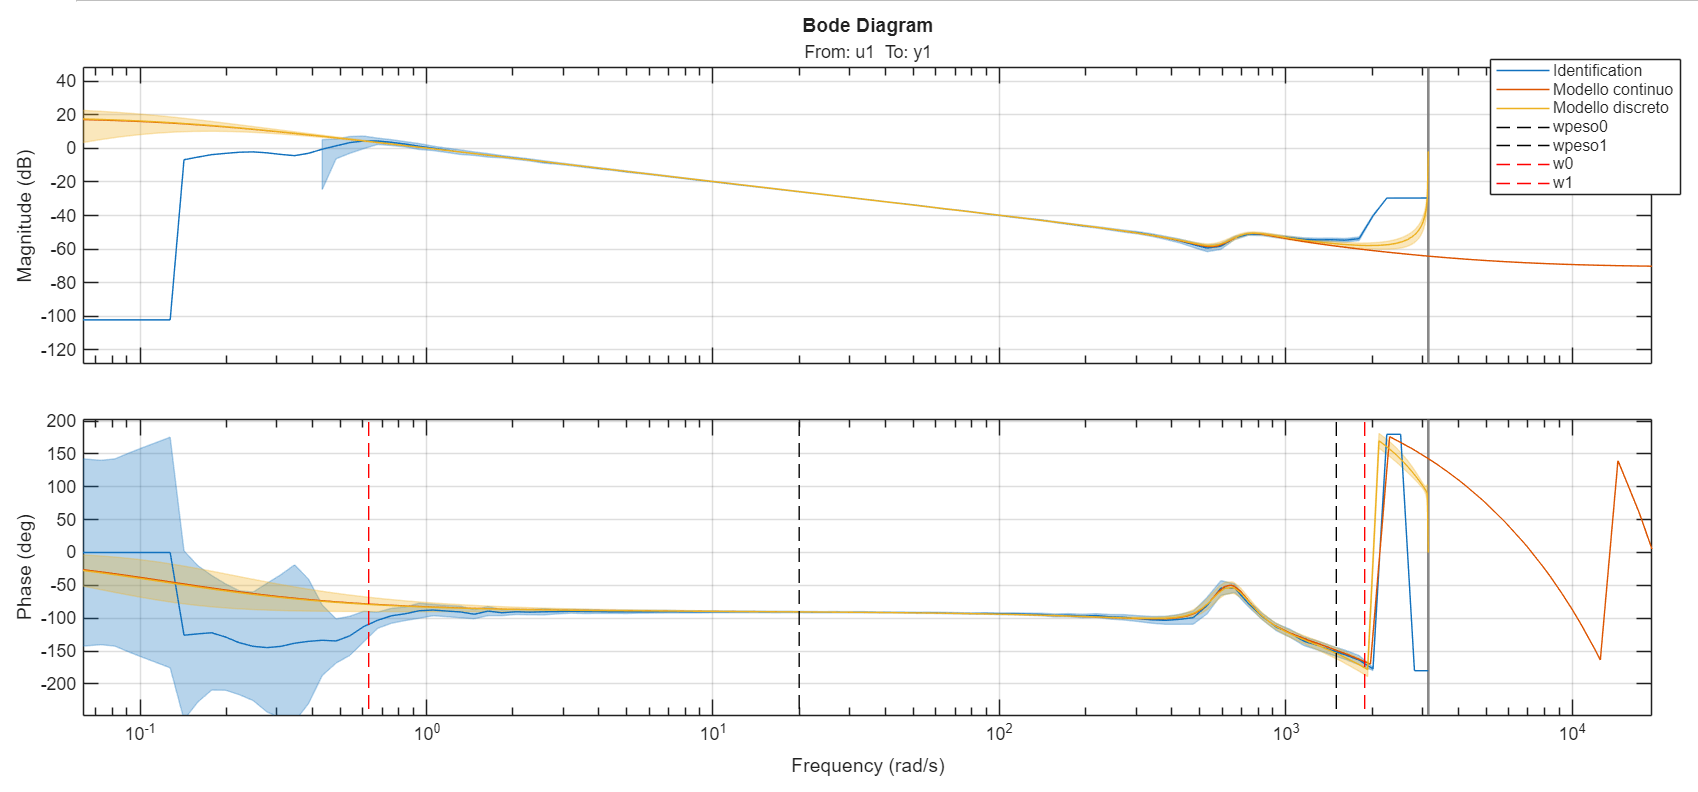
\includegraphics[width=\textwidth]{IMG/ident_valid/J3_IDENTIF_2.png}}
            \caption{Giunto J3 (T04)}
            \label{fig:j3_ident_new}
        \end{subfigure}
    }
    
    \caption{Risultati dell'identificazione per i tre giunti. Si noti il confronto per il giunto J3 tra il test T03 e il test ripetuto T04.}
    \label{fig:all_ident}
\end{figure}

Lo svolgimento delle prove ha richiesto in primo luogo la definizione di una banda di frequenze adeguata,
 al fine di eccitare la dinamica dei giunti senza indurre saturazioni, 
ponendo particolare attenzione nell'identificare i picchi di risonanza e anti-risonanza. Posizionando i pesi almeno una decade al di sotto e al 
di sopra di questi picchi, è stato possibile ottenere una stima più accurata della dinamica del sistema, in prove successive
per ottenere prestazioni una $\omega_c$ migliore identificheremo una finestra dei pesi più precisa.

In prima battuta, i modelli ottenuti nei Test T01, T02 e T03 presentavano una buona coerenza generale, pur evidenziando alcune 
discrepanze in corrispondenza delle frequenze di risonanza. In particolare, come si osserverà nella fase di validazione, 
il modello iniziale del giunto J3 (T03) risultava inadeguato. 

È stato pertanto necessario iterare la procedura di identificazione per questo specifico giunto (Test T04). 
Si è proceduto a ridurre l'ampiezza dell'ingresso, risultata eccessiva rispetto a quella dei giunti precedenti, 
stringendo contemporaneamente lo spettro del segnale chirp e aumentando la durata della prova per migliorare la stima in frequenza.
Infine, si è incrementato l'ordine del modello per catturare in modo più accurato la complessa dinamica del giunto.

Nella seguenti rappresentazioni (Figura \ref{fig:valid_j1_j2}) si possono osservare i risultati di validazione 
per i giunti J1 e J2.

\begin{figure}[H]
    \makebox[\linewidth][c]{
        % Riga J1
        \begin{subfigure}[b]{0.36\textwidth}
            \centering
            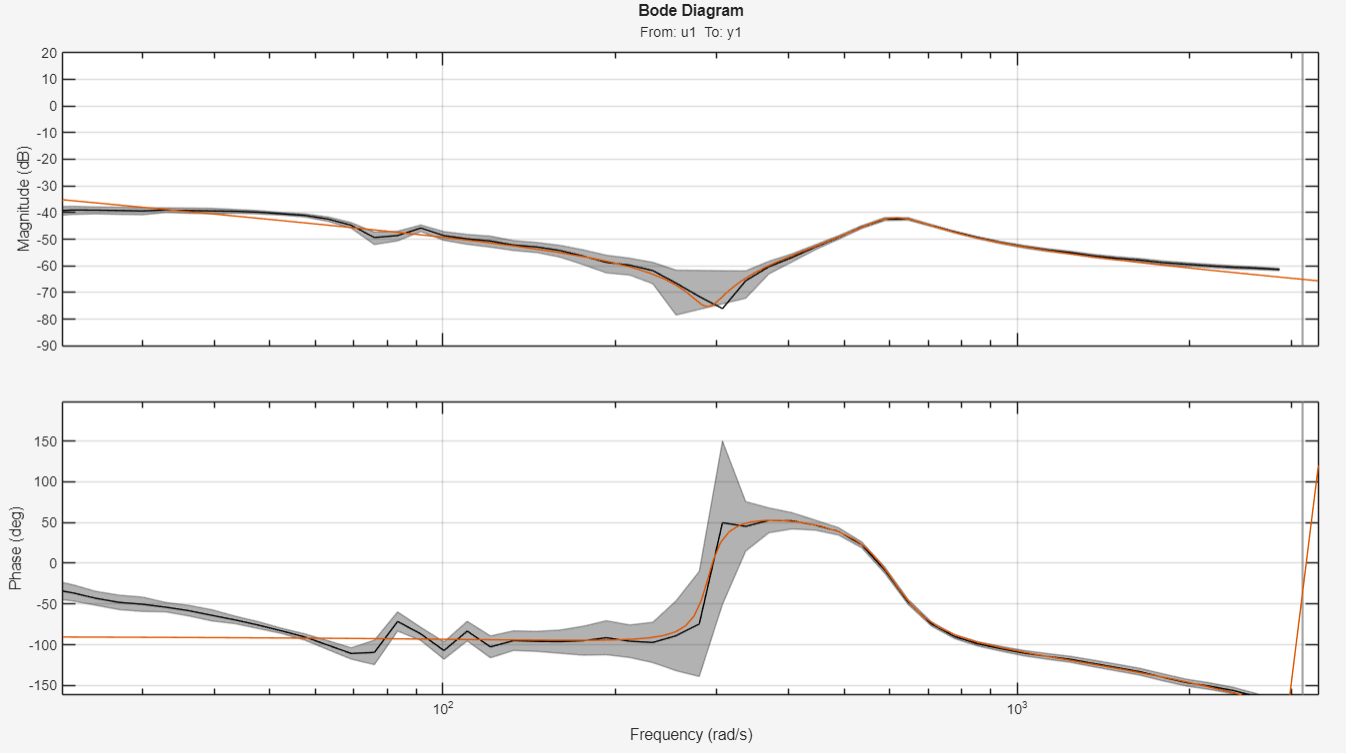
\includegraphics[width=\textwidth]{IMG/ident_valid/J1_1_valid.png}
            \caption{J1 - Validazione 1}
        \end{subfigure}
        \hspace{0.015\textwidth}
        \begin{subfigure}[b]{0.36\textwidth}
            \centering
            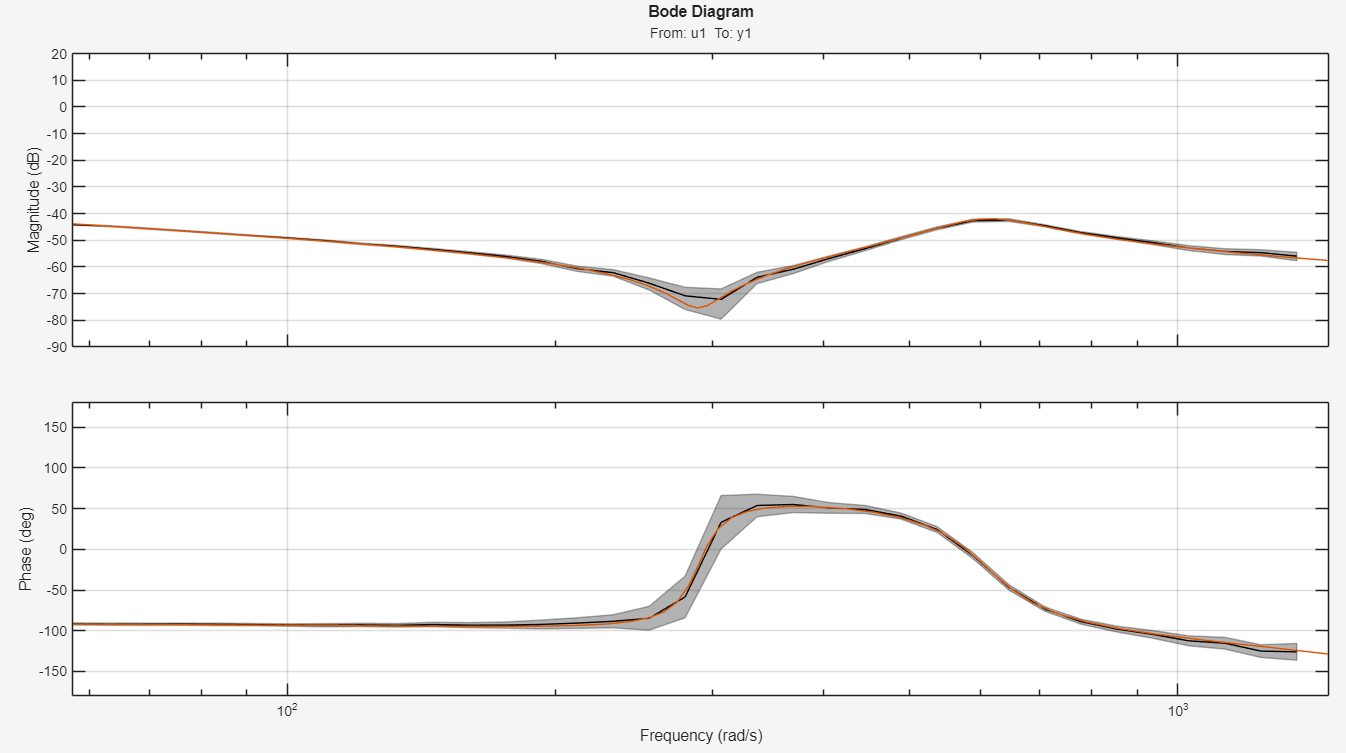
\includegraphics[width=\textwidth]{IMG/ident_valid/J1_2_valid.png}
            \caption{J1 - Validazione 2}
        \end{subfigure}
        \hspace{0.015\textwidth}
        \begin{subfigure}[b]{0.36\textwidth}
            \centering
            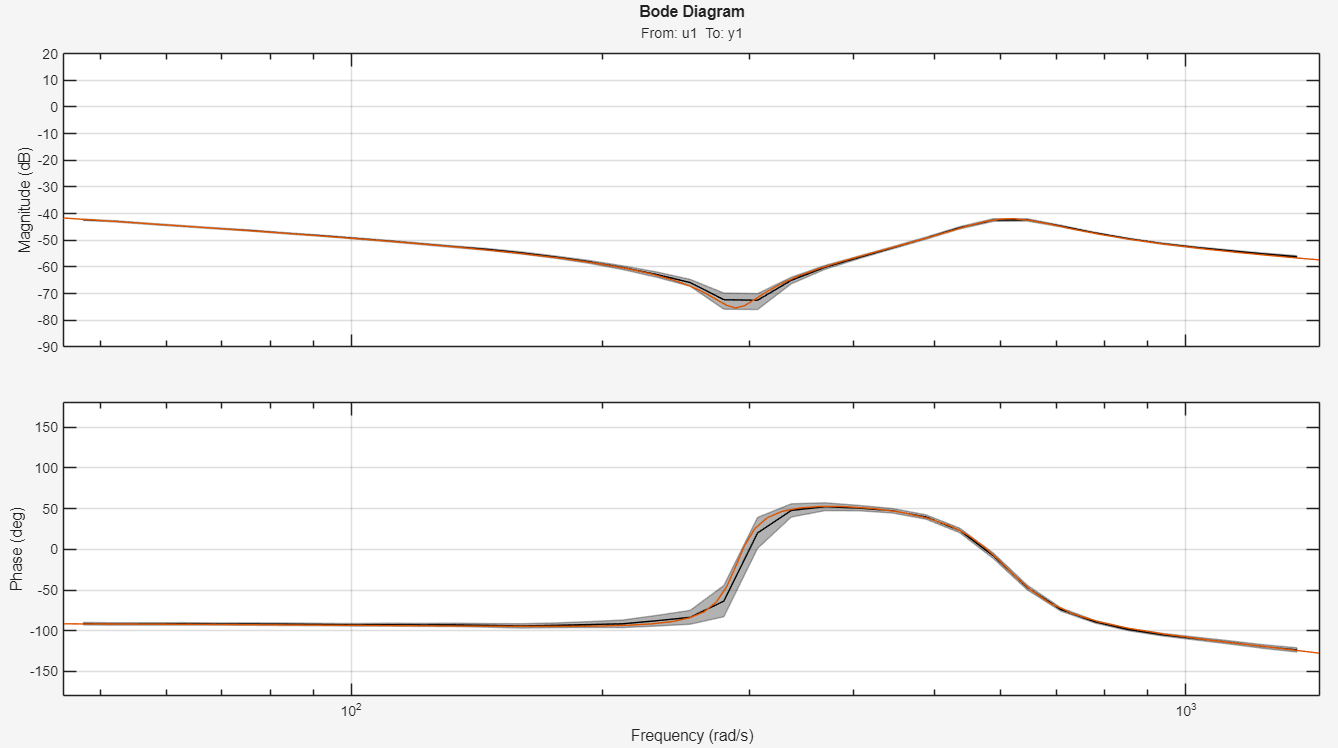
\includegraphics[width=\textwidth]{IMG/ident_valid/J1_3_valid.png}
            \caption{J1 - Validazione 3}
        \end{subfigure}
    }
    
    \vspace{0.3cm}
    
    \makebox[\linewidth][c]{
        % Riga J2
        \begin{subfigure}[b]{0.36\textwidth}
            \centering
            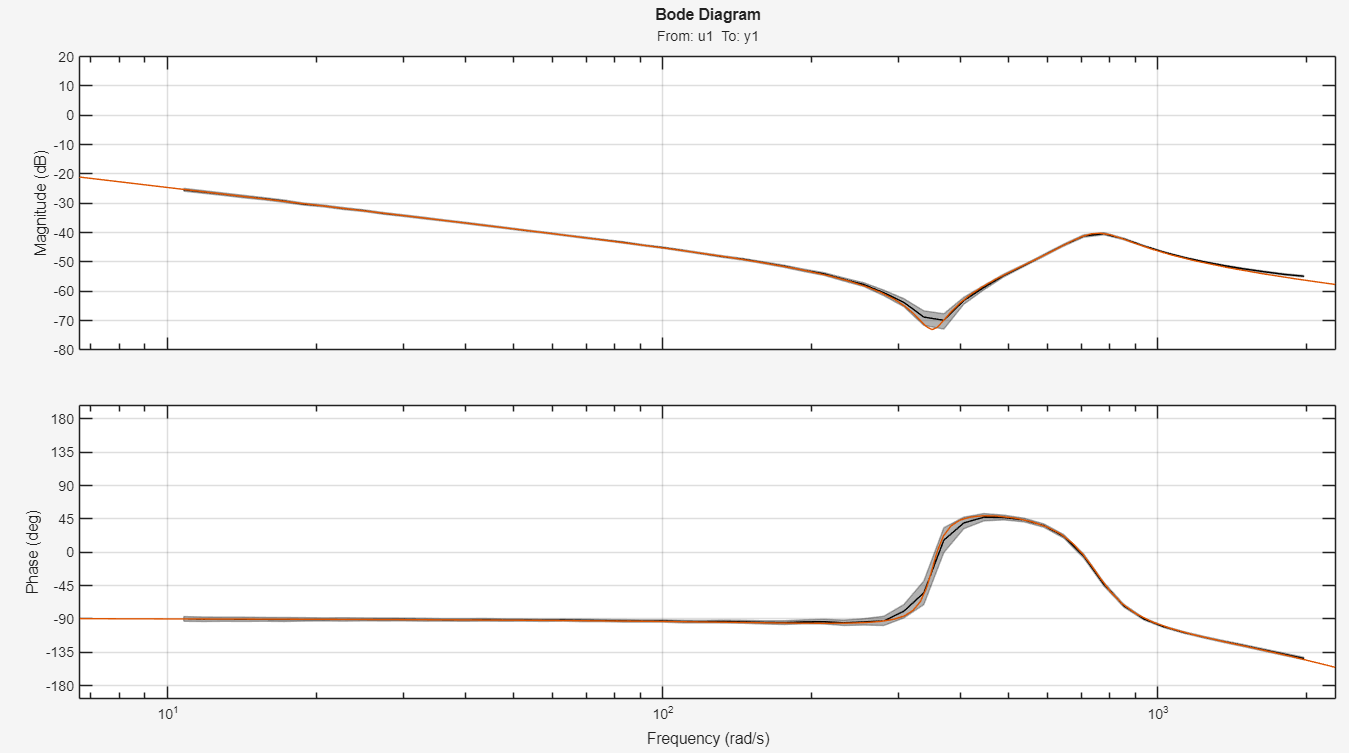
\includegraphics[width=\textwidth]{IMG/ident_valid/J2_1_valid.png}
            \caption{J2 - Validazione 1}
        \end{subfigure}
        \hspace{0.015\textwidth}
        \begin{subfigure}[b]{0.36\textwidth}
            \centering
            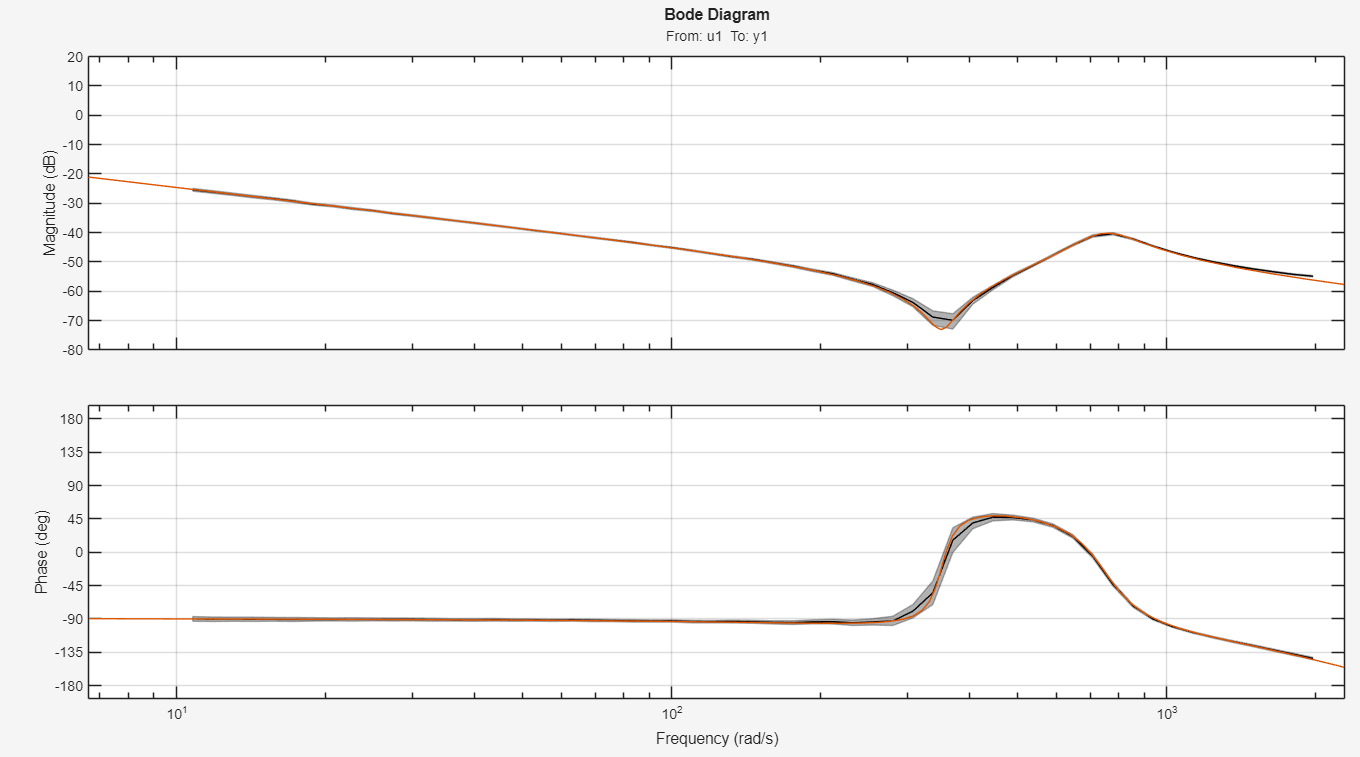
\includegraphics[width=\textwidth]{IMG/ident_valid/J2_2_valid.png}
            \caption{J2 - Validazione 2}
        \end{subfigure}
        \hspace{0.015\textwidth}
        \begin{subfigure}[b]{0.36\textwidth}
            \centering
            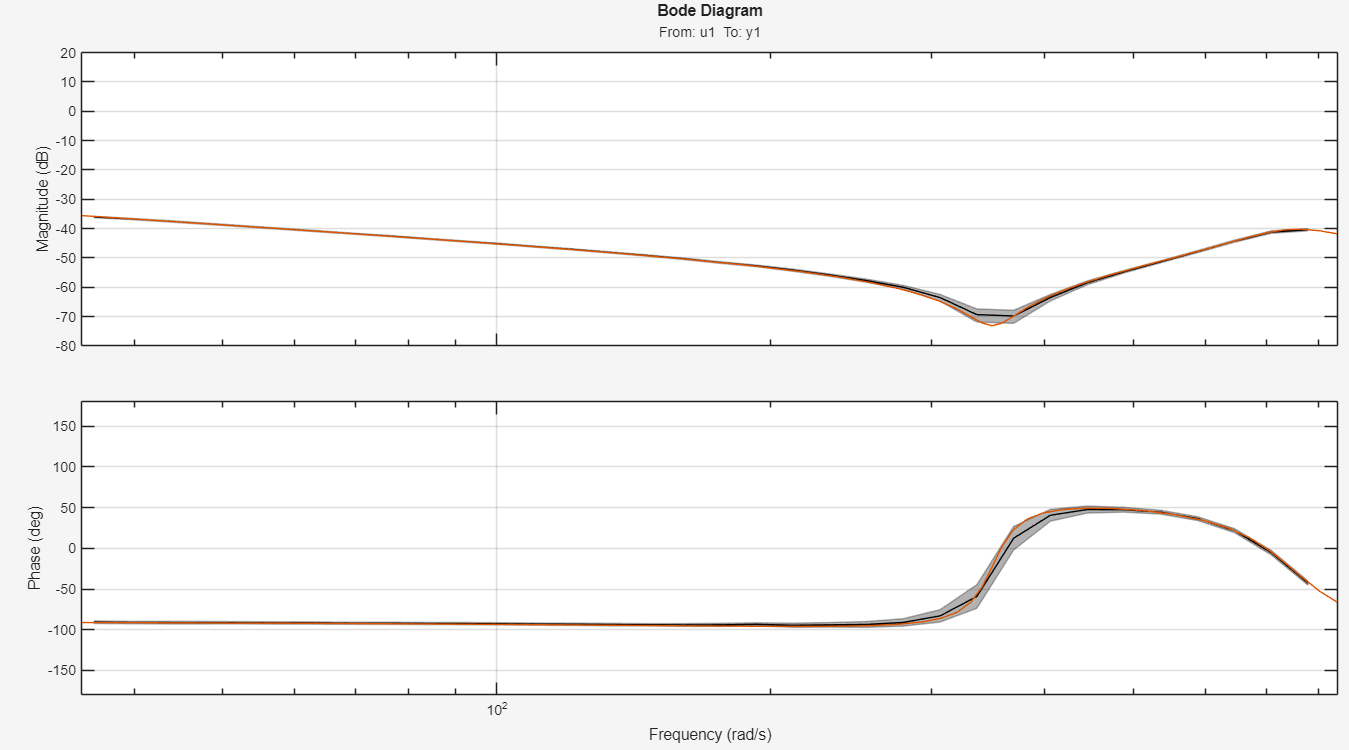
\includegraphics[width=\textwidth]{IMG/ident_valid/J2_3_valid.png}
            \caption{J2 - Validazione 3}
        \end{subfigure}
    }
    
    \caption{Validazione per J1 e J2 in differenti punti di lavoro.}
    \label{fig:valid_j1_j2}
\end{figure}

Per il giunto J3 (Figura \ref{fig:valid_j3}) andando a provare una validazione su tutto lo spettro del chirp 
utilizzando il modello iniziale (T03), si riscontra una grave incongruenza tra la predizione del modello e 
l'effettiva risposta del sistema. 
Utilizzando il modello ottenuto con il (T04), è possibile osservare il livello di confidenza risulta peggiore.
Tuttavia, l'andamento del modello teorico segue in maniera nettamente superiore la risposta reale del sistema, 
giustificando la scelta di utilizzare quest'ultimo modello per le successive fasi di controllo.

\begin{figure}[H]
    \makebox[\linewidth][c]{
        \begin{subfigure}[b]{0.36\textwidth}
            \centering
            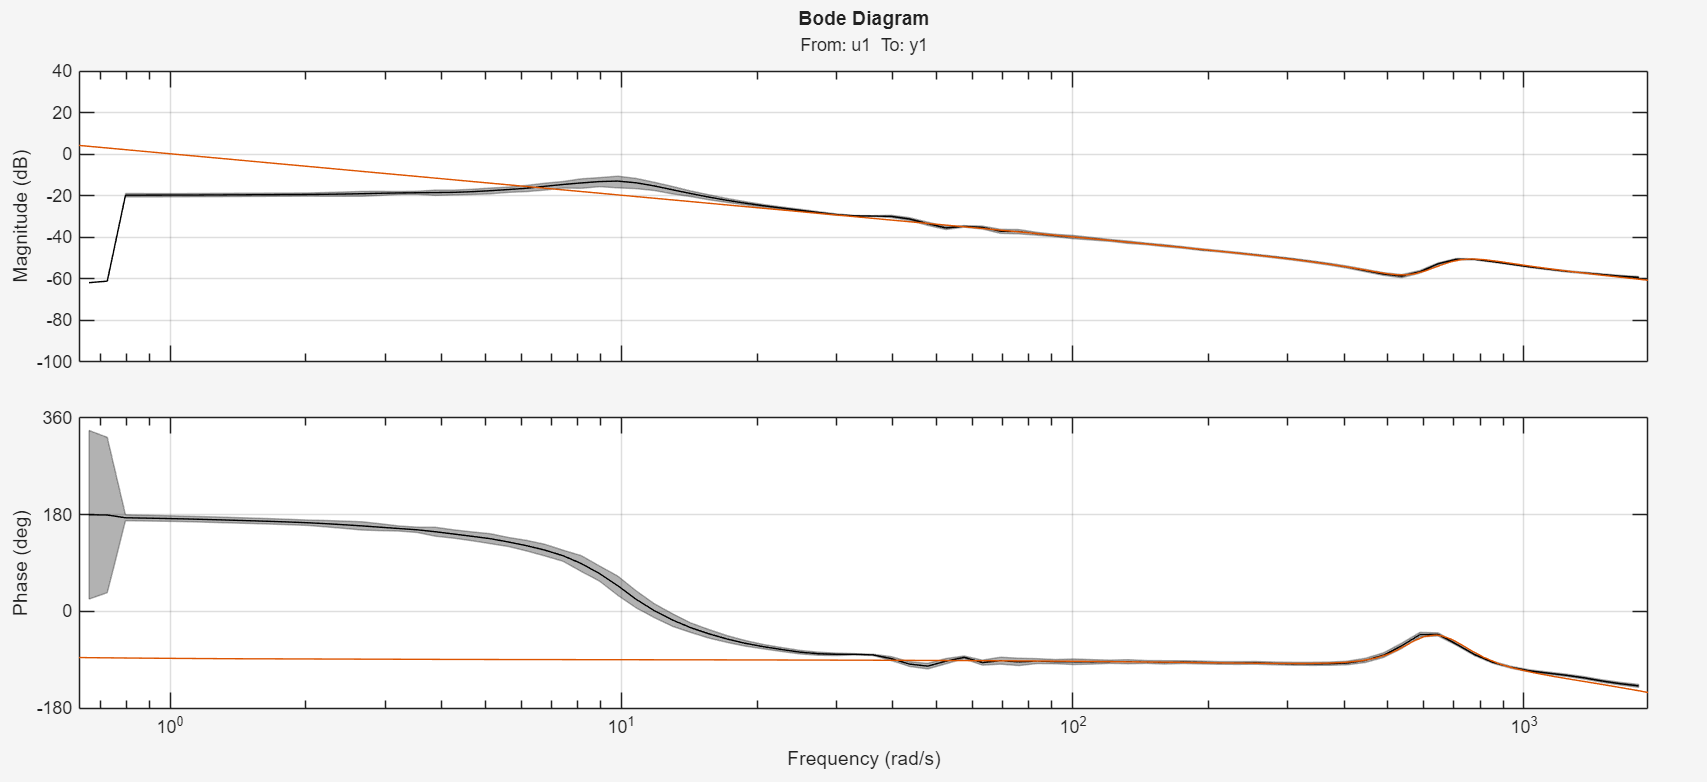
\includegraphics[width=\textwidth]{IMG/ident_valid/J3_1_valid_1.png}
            \caption{J3 (T03)}
            \label{fig:j3_a}
        \end{subfigure}
        \hspace{0.015\textwidth}
        \begin{subfigure}[b]{0.36\textwidth}
            \centering
            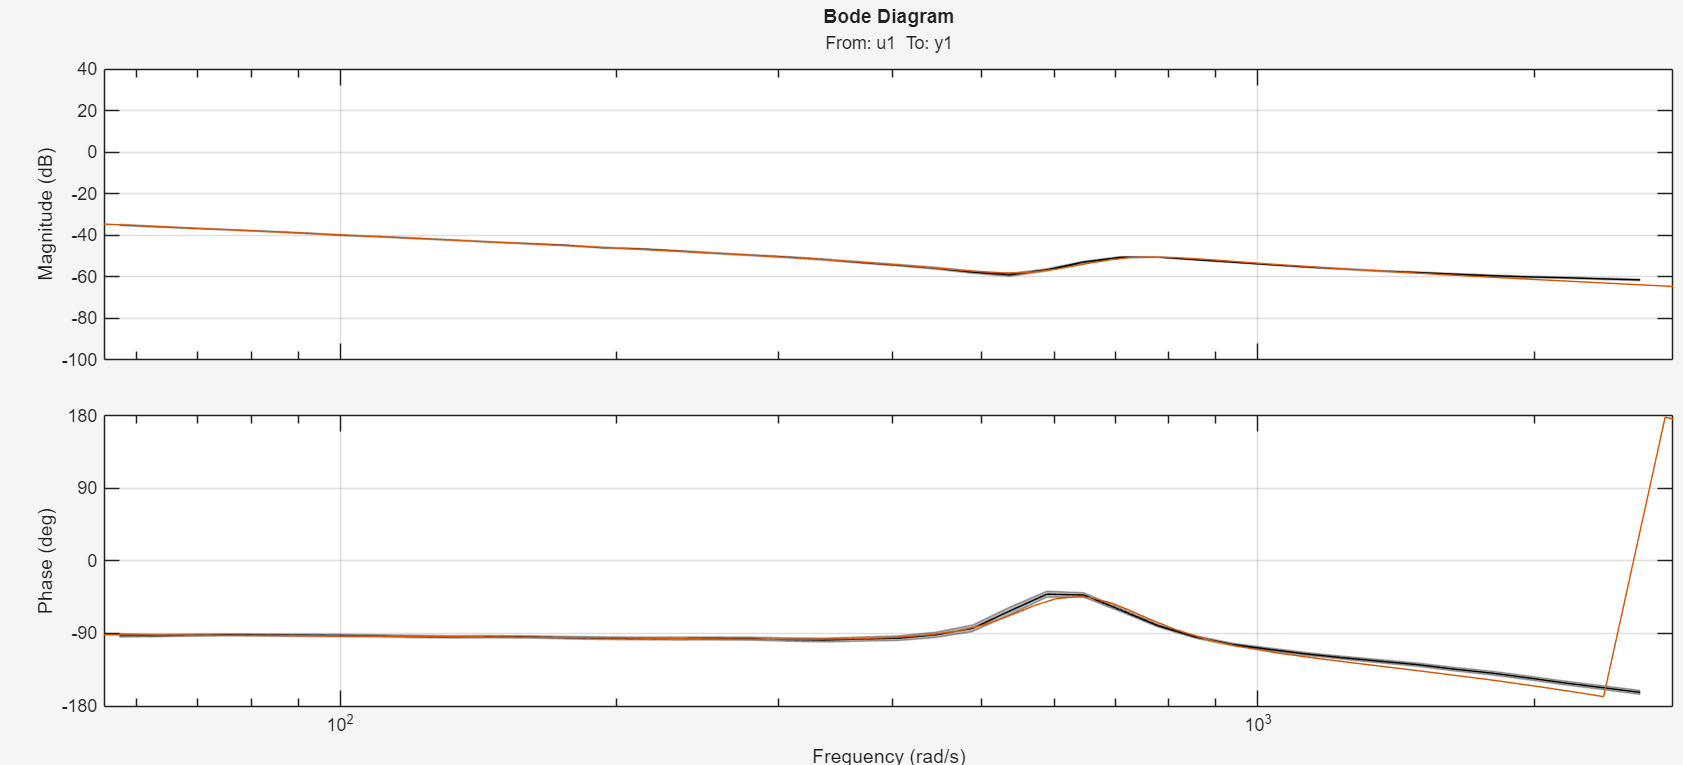
\includegraphics[width=\textwidth]{IMG/ident_valid/J3_2_valid_1.png}
            \caption{J3 (T04)}
            \label{fig:j3_b}
        \end{subfigure}
        \hspace{0.015\textwidth}
        \begin{subfigure}[b]{0.36\textwidth}
            \centering
            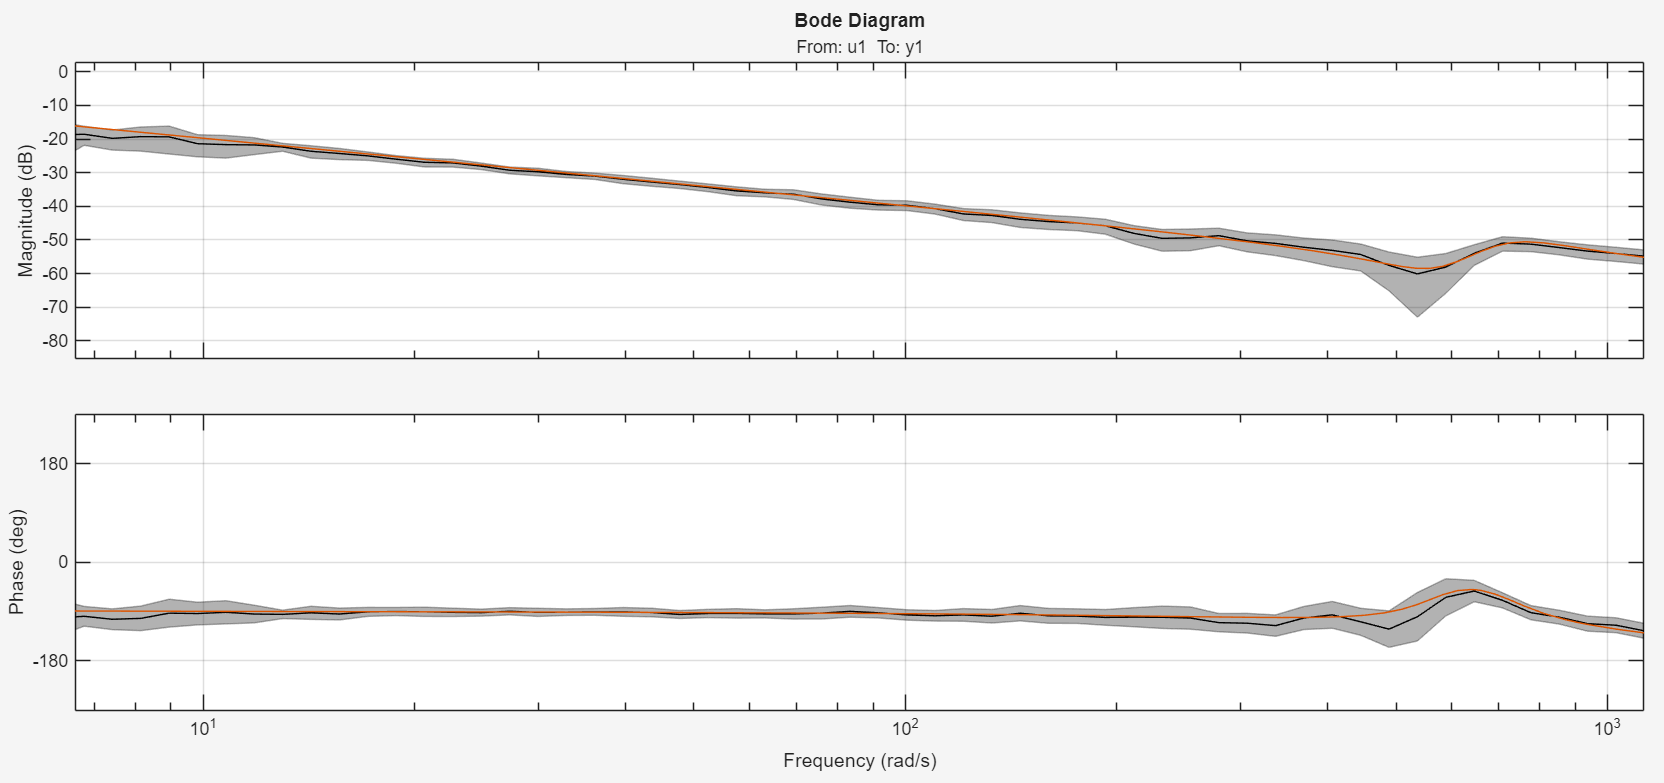
\includegraphics[width=\textwidth]{IMG/ident_valid/J3_2_valid_2.png}
            \caption{J3 (T04)}
            \label{fig:j3_c}
        \end{subfigure}
    }
    
    \caption{Confronto sui test di validazione del J3. Nella fig.(\ref{fig:j3_a}) disallineamento sul modello T03. 
    Nelle fig.(\ref{fig:j3_b}, \ref{fig:j3_c}) tracking nominale del modello T04 migliorato.}
    \label{fig:valid_j3}
\end{figure}

\section{Taratura Manuale, Filtro Notch e Feedforward}
La fase iniziale di progetto del sistema di controllo è stata impostata adottando una classica architettura in cascata, separando chiaramente i compiti:
\begin{itemize}
    \item un \textbf{anello interno di velocità}, controllato da un regolatore PI (Proporzionale-Integrale) per garantire una reiezione rapida dei disturbi;
    \item un \textbf{anello esterno di posizione}, governato da un controllore prevalentemente P (Proporzionale), con dinamiche volutamente più lente.
\end{itemize}

\subsection*{Prime prove e taratura approssimata}
In primis, è stata effettuata una taratura del tutto spannometrica e approssimata, il cui scopo principale era verificare la corretta implementazione e interazione della compensazione feedforward. Va infatti precisato che l'azione di feedforward era stata erroneamente mantenuta attiva fin dall'inizio delle prove, influenzando la dinamica di base.

I parametri dinamici necessari al feedforward sono stati calcolati eseguendo inizialmente lo script \texttt{identificazione\_parametri\_dinamici\_calclo\_T}. Successivamente, lo script \texttt{identificazione\_parametri\_dinamici} è stato eseguito ciclicamente ad ogni modifica strutturale importante, ottenendo così una prima bozza del controllore.

Al fine di garantire che il controllo non risultasse eccessivamente aggressivo nelle fasi preliminari, i parametri di guadagno e i limiti cinematici sono stati impostati su valori fortemente conservativi. Nella Tabella \ref{tab:taratura_manuale} è riportato il confronto tra i parametri di base e quelli utilizzati per il primo test funzionale.

\begin{table}[H]
    \centering
    \footnotesize
    \caption{Confronto parametri tra configurazione Base e Test 1 (taratura manuale conservativa).}
    \label{tab:taratura_manuale}
    \begin{tabular}{lcc | lcc}
    \toprule
    \textbf{Parametro Limite} & \textbf{Base} & \textbf{Test 1} & \textbf{Parametro Guadagno} & \textbf{Base} & \textbf{Test 1} \\
    \midrule
    \texttt{max\_velocity\_j1} & 0.5 & 0.35 & \texttt{joint1\_inner\_Kp} & 25.0 & 25.0 \\
    \texttt{max\_velocity\_j2} & 0.5 & 0.35 & \texttt{joint1\_inner\_Ki} & 2.0  & 2.0 \\
    \texttt{max\_velocity\_j3} & 0.5 & 0.35 & \texttt{joint1\_outer\_Kp} & 5.0  & 5.0 \\
    \texttt{max\_accel\_j1}    & 0.1 & 0.2  & \texttt{joint2\_inner\_Kp} & 50.0 & 40.0 \\
    \texttt{max\_accel\_j2}    & 0.1 & 0.2  & \texttt{joint2\_inner\_Ki} & 1.0  & 1.0 \\
    \texttt{max\_accel\_j3}    & 0.1 & 0.2  & \texttt{joint2\_outer\_Kp} & 5.0  & 5.0 \\
    & & & \texttt{joint3\_inner\_Kp} & 30.0 & 25.0 \\
    & & & \texttt{joint3\_inner\_Ki} & 15.0 & 5.0 \\
    & & & \texttt{joint3\_outer\_Kp} & 15.0 & 10.0 \\
    \bottomrule
    \end{tabular}
\end{table}

I risultati di questa prima prova sono visibili in Figura \ref{fig:par_din_manuale}. Avendo imposto limiti di velocità molto bassi, i segnali di velocità acquisiti risultavano di entità ridotta. Di conseguenza, il rapporto segnale/rumore si è rivelato critico: il segnale grezzo riportava una componente di disturbo ad alta frequenza molto marcata. Inoltre, una grave mancanza che ha limitato le velocità massime raggiungibili in queste prime prove è imputabile all'inadeguatezza del modello iniziale utilizzato per il giunto J3.

\begin{figure}[H]
    \centering
    \begin{subfigure}[b]{0.48\textwidth}
        \centering
        
\includegraphics[width=\textwidth]{IMG/taratura_manuale/Calcolo_ParDin_1A.png}
        \caption{Risposta dinamica 1A}
    \end{subfigure}
    \hfill
    \begin{subfigure}[b]{0.48\textwidth}
        \centering
        
\includegraphics[width=\textwidth]{IMG/taratura_manuale/Calcolo_ParDin_1B.png}
        \caption{Risposta dinamica 1B}
    \end{subfigure}
    \caption{Prove eseguite con controllore tarato manualmente in modalità conservativa. Si nota la marcata presenza di rumore dovuta alle basse velocità di test.}
    \label{fig:par_din_manuale}
\end{figure}

\subsection*{Studio della banda passante ed evoluzione dei guadagni}
Superata la fase preliminare, si è proceduto alla taratura manuale dell'anello interno. Fissata la dinamica coppia-velocità, è stata imposta una pulsazione di taglio $\omega_c$ target. 
Sfruttando il giunto J1 come riferimento, sono state testate tre condizioni principali:
\begin{itemize}
    \item $\omega_c = 20$ rad/s: comportamento molto robusto ma eccessivamente conservativo (Margine di Fase molto alto, circa $86^\circ$).
    \item $\omega_c = 30$ rad/s: un buon compromesso tra reattività e robustezza.
    \item $\omega_c = 60$ rad/s: comparsa di criticità in prossimità dei picchi risonanti (con pericolosi avvicinamenti allo 0 dB), riducendo i margini di stabilità pratici.
\end{itemize}

Questa indagine ha guidato la scelta verso un \textit{inner loop} più aggressivo ma pur sempre robusto ($\omega_c \approx 30$ rad/s), portando i guadagni a valori sensibilmente più alti rispetto alla "Test 1" (es. J1: $K_p \approx 79.6$, $K_i \approx 119.3$; J2: $K_p \approx 51.4$, $K_i \approx 77.1$; J3: $K_p \approx 29.1$, $K_i \approx 43.7$).

Parallelamente, l'anello esterno è stato accordato applicando la regola empirica della separazione delle decadi (banda passante circa $1/10$ di quella interna), impostando unicamente l'azione proporzionale ($K_p$ tra $2.0$ e $3.0$) e azzerando l'azione integrale. Questa accortezza ha minimizzato le interazioni indesiderate tra i due anelli.

\subsection*{Introduzione del Filtro Notch}
Con l'aumento delle prestazioni, l'analisi in frequenza ha reso palese l'effetto destabilizzante delle risonanze elastiche della meccanica (SEA). Per mitigare il problema è stato introdotto un \textbf{Filtro Notch} nel ramo più sensibile al contenuto ad alta frequenza (\texttt{filters\_on\_derivative\_error}).

Il filtro è stato centrato in corrispondenza del picco risonante dominante di ciascun giunto, impostando gli smorzamenti ($\xi_z, \xi_p$) in modo da bilanciare la profondità di attenuazione e la robustezza, evitando notch eccessivamente stretti che risulterebbero sensibili alle incertezze parametriche. Tipici valori utilizzati sono stati:
\begin{itemize}
    \item \textbf{J1:} $\omega_n \approx 620$ rad/s, $\xi_z \approx 0.1$, $\xi_p \approx 0.4$
    \item \textbf{J2:} $\omega_n \approx 750$ rad/s, $\xi_z \approx 0.1$, $\xi_p \approx 0.4$
\end{itemize}

\section{Taratura Ottimale}
L'approccio manuale descritto in precedenza si è rivelato fondamentale per delineare i limiti della dinamica reale: ha permesso di isolare le bande critiche, quantificare l'esigenza dei filtri notch e individuare nel modello del giunto J3 il vero collo di bottiglia dell'intero sistema. Risolta l'incongruenza su J3 tramite una ri-identificazione, il passaggio alla sintesi tramite ottimizzazione analitica è risultato naturale.

Sfruttando lo script \texttt{taratura\_ottima.mlx}, il problema di controllo è stato riformulato imponendo vincoli espliciti su:
\begin{itemize}
    \item \textbf{Robustezza:} imposizione di limiti sul picco della funzione di sensibilità ($M_s$) e sul Margine di Fase ($PM$).
    \item \textbf{Reiezione disturbi:} attenuazione richiesta a bassa frequenza (es. $\approx 0.15$ per $\omega < 2$ rad/s).
    \item \textbf{Attenuazione rumore:} abbattimento del guadagno ad alta frequenza (es. $\approx 0.1$ per $\omega > 400$ rad/s).
\end{itemize}

\section{Simulazioni e confronto prestazionale}

\section{Configurazione finale e conclusioni}

\end{document}